
\chapter{Teilautomatisierte Generierung von Page Objects}
\label{sec:teilautomatisierte_generierung_von_pageObjects}

Ein großer Teil des in Kapitel \ref{sec:probleme_des_page_object_pattern} angesprochenen initialen Mehraufwands bei der Verwendung des Page Object Pattern beläuft sich auf die Erstellung der Page Objects.
Wie in Listing \ref{lst:poCreatePage} und \ref{lst:poShowPage} zu sehen ist, handelt es sich bei Page Objects jedoch um wenig komplexe Klassen. In der Praxis zeigt sich, dass ein Großteil der Arbeit darin besteht die verschiedenen Locatoren der Elemente aus dem Quelltext der Seite herauszufinden und in die generische Form eines Page Objects zu überführen.
Diese Arbeit kostet zwar viel Zeit, ist allerdings nicht gerade anspruchsvoll.
Möchte man den initialen Mehraufwand bei der Verwendung des Page Object Pattern entgegenwirken bieten die Page Objects somit einen guten Ansatzpunkt.
Ihre Erstellung ist zeitaufwendig und weitestgehend generisch. Gute Voraussetzungen also um das Erzeugen der Pagae Objects zu Automatisieren.
\section{Übersicht über die Idee}
\label{sec:uebersicht_ueber_idee}


Selenium in Verbindung mit dem Page Object Pattern ist auch ein Teil des Technologiestacks des IT-Dienstleisters der Landeshauptstadt München (it@M) und wird dort zum Testen komplexer Webanwendungen verwendet. Auch bei it@M hat man in Bezug auf die Erstellung der Page Objects die Erfahrungen gemacht, dass es sich um eine generische und zeitaufwendige Arbeit handelt.
In Zusammenarbeit mit it@M wurde daher die Idee entwickelt, das Erstellen von Page Objects mit Hilfe einer Softwarelösung zu unterstützen. 
Anhand des Seitenquelltextes der zu testenden Webanwendung sollen die verschiedenen Elemente des Page Objects identifiziert und zur Generierung der Page Objects verwendet werden.
Zwei Ansätze wurden dabei diskutiert. Eine vollautomatisierte Generierung von Page Objects und eine teilautomatisierte Generierung.
Ein vollautomatischer Ansatz würde beinhalten, dass für einen übergebenen Seitenquelltext ohne weiteres Zutun ein vollständiges Page Object generiert wird. Dieser Ansatz hat jedoch mit zahlreichen Problemen zu kämpfen. Oft wird nur ein Bruchteil der Elemente einer Webseite für die Testfälle benötigt. Selenium kann aber prinzipiell jedes Element, dass im Seitenquelltext bereitgestellt wird, ansprechen. Bei einer vollautomatischen Generierung müssten daher entweder alle Elemente einer Seite übernommen oder eine definierte Auswahl getroffen werden.
Wird eine Auswahl getroffen besteht das Risiko, dass Elemente ausgelassen werden die vom Tester möglicherweise benötigt werden. Werden alle Elemente übernommen, werden die Page Objects schnell überladen und unübersichtlich. Das Überladen der Page Objects geschieht dann auf Kosten der Robustheit. Strukturelle Änderungen in der Website wirken sich auch auf die Locatoren der Elemente in den Page Objects aus. Um die Page Objects stabil zu halten, müssen diese bei Änderungen in der Seitenstruktur berichtigt werden.
Es ist daher nicht sinnvoll Elemente in den Page Objects zu pflegen, die nicht verwendet werden. Unbenutzte Elemente bedeuten entweder zusätzlichen Wartungsaufwand oder veralten unbemerkt.
Ein weiteres Problem des vollautomatischen Ansatzes stellen die Übergänge zwischen den Seiten einer Webanwendung dar. Interaktionen mit der Webanwendung wie beispielsweise das betätigen eines Button führen oft zum aufrufen einer neuen Seite. Im weiteren werden diese Übergänge als Transitions bezeichnet. Diese Transitions werden optimaler weise auch in den Page Objects abgebildet. Das Page Object gibt dazu das entsprechende Page Object der Zielseite als Rückgabe eines Methodenaufrufs zurück, wie es beispielsweise in der Methode createEntry() im Listing \ref{lst:poCreatePage} gezeigt ist. Allein aus dem Seitenquelltext zu ermitteln welche Seite das Ziel einer Transition ist erweist sich jedoch oft als sehr schwierig bis unmöglich.
Um die Komplexität des Projektes auf Grund der genannten Probleme nicht zu groß werden zu lassen wurde sich für einen teilautomatisierte Lösung entschieden.
Ziel ist es also nicht, automatisch ein vollständiges Page Object zu generieren sondern den Entwickler bei der Generierung der Page Objects zu unterstützen. Anhand des Quelltextes sollen dem Entwickler die möglichen Elemente der Seite in einer Vorauswahl bereitgestellt werden. Aus diesen Elementen können dann diejenigen ausgewählt werden, die vom Entwickler im späteren Page Object benötigt werden. Auf diese Weise wird eine Überladung der Page Objects verhindert und gleichzeitig sichergestellt, dass die Elemente vorhanden sind, die benötigt werden.
Ob es sich bei einem Element um eine Transition handelt, also ein Element welches auf eine neue Seite führt, muss auch nicht mehr automatisch anhand des Quelltextes ermittelt werden sonder kann vom Entwickler direkt bei der Auswahl der benötigten Elemente mit angegeben werden.
Die so vom Entwickler ausgewählten Informationen können dann verwendet werden um daraus das fertige Page Object zu generieren.
Im Rahmen des Projektes SeleniPo soll dieser Ansatz in Zusammenarbeit mit it@M in Form einer Denktopanwendung umgesetzt werden. 

\section{Abgrenzung zu bestehenden Ansätzen}
\label{sec:abgrenzung_zu_bestehenden_ansaetzen}
Sowohl für die vollautomatische Generierung von Page Objects als auch für eine teilautomatisierten Generierung gibt es bereits mögliche Lösungsansätze. 
Stocco et al. \cite{stocco_why_2015} beschreiben in einem Paper das von ihnen entwickeltes Framework APOGEN mit deren Hilfe Page Objects vollautomatisch generiert werden können. Die Generierung der Page Objects soll dabei weit über das Anlegen von Elementen hinausgehen und auch die Funktionalitäten der einzelnen Webseiten in Form von Methoden mit einschließen.
Das Framework analysiert dazu die Struktur der Webanwendung mittels eines Crawlers. Die Informationen die über den Crawler zusammengetragen wurden, wie beispielsweise das DOM der einzelnen Webseiten, werden anschließend über eine statische Analyse aufbereitet und für die Generierung der Page Objects verwendet.
Nach eigenen Angaben sollen ca. 75\% des von APOGEN generierten Codes ohne Anpassungen verwendet werden können. Die restlichen 25\% benötigen nur kleine Änderungen.
Bei APOGEN handelt es sich jedoch um ein noch sehr junges Projekt. Das Paper zu diesem Projekt wurde im Mai 2015 veröffentlicht. APOGEN ist daher eher einen Prototyp der zwar die Möglichkeiten aufzeigt die in diesem Bereich gegeben sind jedoch noch nicht für den produktiven Einsatz in einem großen unternehmen geeignet ist.
Nach eigenen Angaben Leidet das Projekt noch unter einigen Einschränkungen. Eine der genannten Einschränkungen ist die Limitierung durch den Crawler.
APOGEN kann nur Webseiten in Page Objects umwandeln, die auch durch den Crawler erreicht wurden.
Für einfache Webanwendungen stellt das kein großes Problem da, für sehr komplexe Anwendungen mit einer ausgeprägten logischen Validierung allerdings schon.
Viele Seiten die hinter logisch validierten Eingaben liegen können vom Crawler nicht erreicht werden und stehen somit für die Generierung nicht zur Verfügung.

Neben der vollautomatischen Generierung existieren noch eine Reihe von Open-Source-Framworks 
die einen teilautomatisierten Ansatz verfolgen, ähnlich wie es das Projekt SelneiPo erreichen will.
Stocco et al. \cite{stocco_why_2015} nennen in ihrem Paper die drei derzeit wichtigsten Vertreter:

\begin{itemize}
\item \textit{OHMAP} \cite{virtuetech_gmbh_ohmap_2015}: Bei OHMAP handelt es sich um eine online Webseite die es dem Benutzer erlaubt HTML-Code in eine Textarea zu Kopieren. Aus dem übergebenen HTML-Code generiert das Tool eine einfache Java-Klasse die für jedes gefundene Input-Feld ein WebElement enthält. Die Variablennamen werden dabei aus den HTML-Attributen gebildet. Als Locator wird ein einfacher XPath-Ausdruck verwendet.
	
\item \textit{SWD Page Recorder} \cite{dmytro_zharii_dzharii/swd-recorder_2015}: Der SWD Page Recorder ermöglicht es dem Benutzer eine beliebige Webanwendung zu starten und das GUI der Anwendung mit einem click\&record-Mechanismus zu inspizieren.
Nach jedem Klick auf das Interface der Anwendung wird ein drop-down-Menü angezeigt in welches manuell ein Name für das ausgewählte Element angegeben werden kann. Als Locator wird ein einfacher XPath-Ausdruck generiert.
Das so erstellte Modell der Anwendung kann in verschiedene Sprachen exportiert werden, wie beispielsweise Java, C\#, Rython, Ruby oder Perl. Beim SWD Page Recorder handelt es sich um eine .NET Anwendung.

\item\textit{ WTF PageObject Utility Chrome Extension} \cite{daniel_wiredrive/wtframework_2015}: WTF unterstützt den Entwickler beim erstellen von Page Objects indem Locatoren der Form id, name, CSS oder XPath erstellt werden. Der generierte Code ist in Python.
	
\end{itemize}

Der Technologiestack von it@M sieht eine Entwicklung der Selenium-Testfälle in Java vor. Als Betriebssystem kommt darüber hinaus Linux zum Einsatz.
Zwei der genannten Lösungsansetzen scheiden daher von vornherein für den produktiven Einsatz beim externen IT-Dienstleister der Landeshauptstadt München aus. Beim SWD Page Recorder handelt es sich um eine .NET Anwendung die nur schwer unter Linux betrieben werden kann. Die WTF PageObject Utility Chrome Extension kann nur im Python-Umfeld betrieben werden. OHMAP wäre aus technischer Sicht eine mögliche Lösungsalternative. Allerdings sind Komfort und Umfang der Anwendung aus sicht von it@M nicht ausreichend. Ohne eigne Konfiguration ist es mit OHMAP nur möglich input-Felder zu extrahieren.
Der HTML-Quelltext muss händisch aus der zu testenden Anwendung extrahiert werden. \\
OWAP als auch der SWD Page Recorder haben zusätzlich das Problem, dass die erzeugten XPath ausdrücke oft sehr einfach gewählt werden und damit sehr stark von der Position der Element innerhalb der Seite abhängig sind. Die eigentlichen Charakteristika der Elemente werden somit oft nicht beachtet. Listing \ref{lst:badXPath}
zeigt einen solche von OHMAP generierten XPath.

\begin{lstlisting}[caption={Einfacher XPath-Locator des Projektes OHMAP},label={lst:badXPath}]
	public class YourPageObjectName {
		//...		
 		@FindBy(xpath = "/html/body/div/div[1]/div[1]/h1/a[2]")
		public WebElement followVirtuetechGmbH;	
		//...
	}
\end{lstlisting}

Der zu adressierende Link in  Listing \ref{lst:badXPath} wird alleine über seine Position innerhalb des DOM der Seite bestimmt.
Um den Locator zu zerstören würde es genügen ein weiteres div-Tag vor dem Link einzufügen.
\\
Ein weiteres Problem, dass sich die gezeigten Lösungen teilen ist, dass sie immer nur ein Page Object auf einmal betrachten. Transitionen, also Übergänge zwischen den einzelnen Webseiten der zu testenden Anwendung, werden somit nicht beachtet. Die dynamische Komponente der Anwendung wird beim generieren der Page Objects somit außer acht gelassen und muss nachträglich händisch hinzugefügt werden.

Mit SeleniPo soll der Versuch unternommen werden die Schwachstellen der bereits existierenden Lösungsansätzen zu verbessern und eine Plattformunabhängige Lösung zu schaffen, die in der IT-Infrastruktur von it@M betrieben werden kann.

\newpage
\section{SeleniPo - Page Object Generator}
\label{sec:selenipo_pogenerator}

Abbildung \ref{fig:poGenerator} zeigt die Denktopanwendung (Page Object Generator) die im Rahmen des Projektes SeleniPo entwickelt wurde. Mit Hilfe dieser Anwendung ist es möglich Page Objects teilautomatisiert zu generieren. Die Anwendung bietet dazu die Möglichkeit einen Browser zu starten und über vorgefertigte Selektoren die Webanwendung nach benötigten Elementen bzw. Transitionen zu durchsuchen. Auf diese Weise kann ein Modell der Anwendung erstellt werden, dass zur Generierung der Page Objects verwendet wird.

\begin{figure}[htb]
  \centering  
  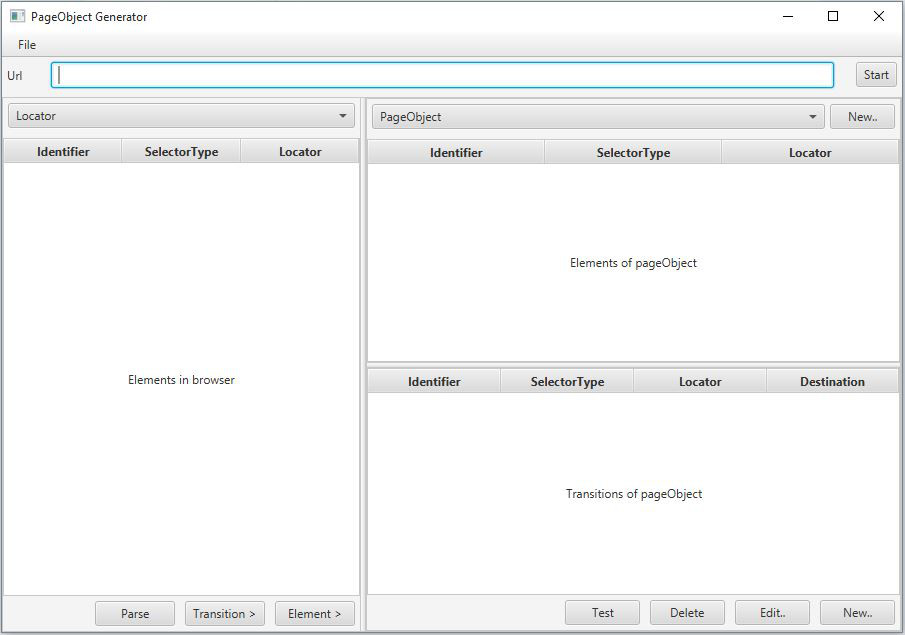
\includegraphics[scale=0.5]{img/poGenerator.JPG}\\
  \caption{SeleniPo - Page Object Generator}
  \label{fig:poGenerator}
\end{figure}



Das Interface des Page Object Generators teilt sich in drei Bereiche:

\begin{itemize}
	\item Das aktuelle Page Object Modell (Abbildung \ref{fig:poGeneratorPo})
	\item Den HTML-Parser (Abbildung \ref{fig:poGeneratorHtml})
	\item Das Menü (Abbildung \ref{fig:poGeneratorMenu})
\end{itemize}


Abbildung \ref{fig:poGeneratorPo} zeigt den Bereich des Generators mit dem das aktuelle Page Object Modell der zu testenden Anwendung verwaltet werden kann. Mit diesem Bereich der Anwendung können neue Page Objects angelegt und bearbeitet werden. Elemente und Transitionen können manuell hinzugefügt, editiert oder gelöscht werden. Darüber hinaus bietet Die Anwendung die Möglichkeit existierende Elemente und Transitionen auf ihre Richtigkeit zu testen.

\begin{figure}[htb]
  \centering  
  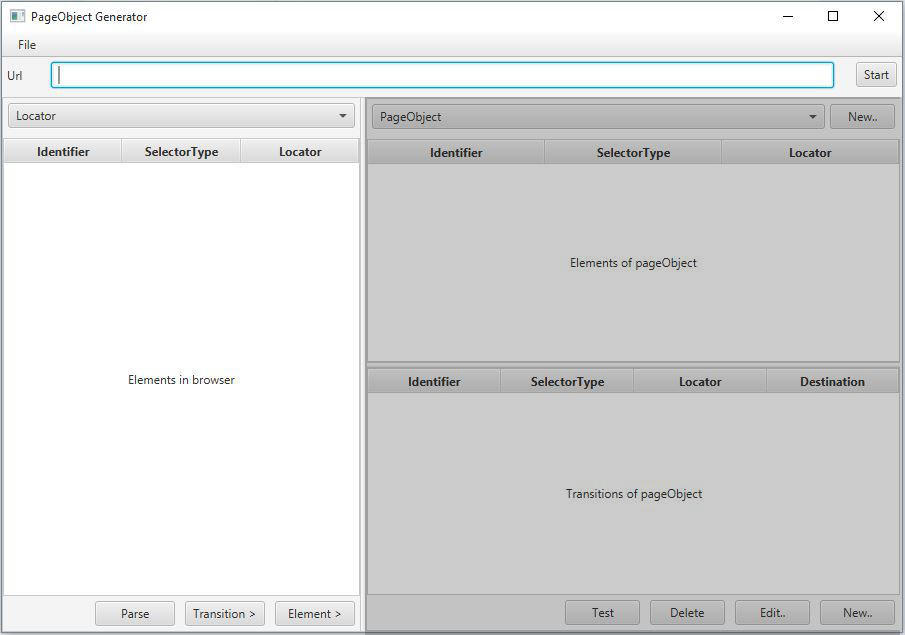
\includegraphics[scale=0.5]{img/poGeneratorPo.JPG}\\
  \caption{SeleniPo - Page Object Generator - Page Object Model}
  \label{fig:poGeneratorPo}
\end{figure}

\newpage

Abbildung \ref{fig:poGeneratorHtml} zeigt den Bereich des Generators mit dem der Entwickler bei der Erstellung von Elementen und Transitionen im Page Object unterstützt werden kann.
Über den Button Start kann ein Browser gestartet werden. Über das Locator-Dropdown kann dann über vorgefertigte Selektoren die aktuell im Browser dargestellte Webseite nach Elementen bzw. Transitionen durchsucht werden. Im Page Object benötigte Elemente und Transitionen können dann in das ausgewählte Page Object im Page Object Modell übernommen werden.

\begin{figure}[htb]
  \centering  
  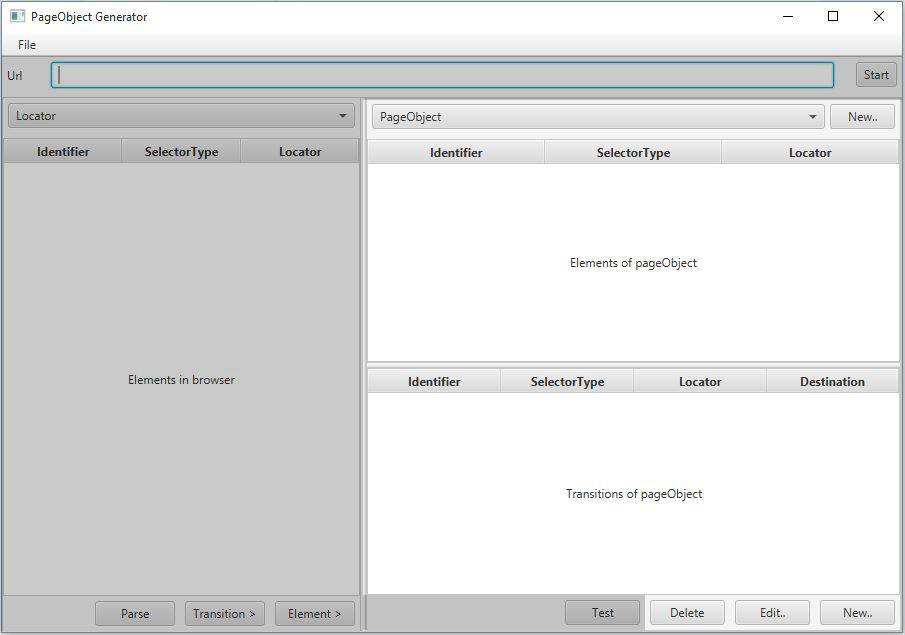
\includegraphics[scale=0.5]{img/poGeneratorHtml.JPG}\\
  \caption{SeleniPo - Page Object Generator - Html Parser}
  \label{fig:poGeneratorHtml}
\end{figure}

\newpage

Abbildung \ref{fig:poGeneratorMenu} markiert das Menü des Page Object Generator. Mit Hilfe des Menüs können Zwischenstände des Page Object Modells gespeichert und geladen werden.
Über das Menü kann darüber hinaus die Generierung der Page Objects aus dem aktuell geladenen Modell gestartet werden.

\begin{figure}[htb]
  \centering  
  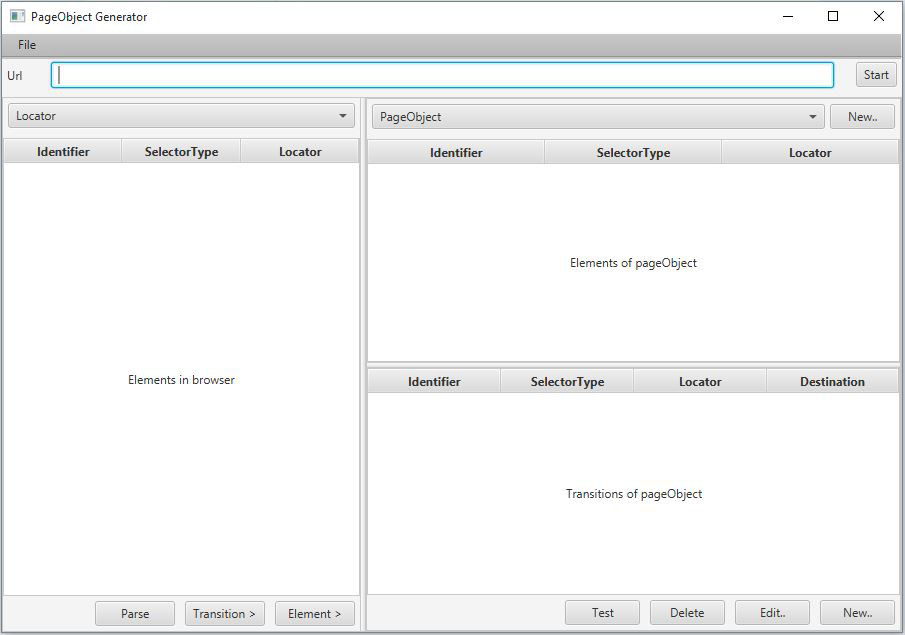
\includegraphics[scale=0.5]{img/poGeneratorMenu.JPG}\\
  \caption{SeleniPo - Page Object Generator - Menü}
  \label{fig:poGeneratorMenu}
\end{figure}

\subsection{Deploymentsicht}

\label{sec:deploymentsicht}
\begin{figure}[htb]
  \centering  
  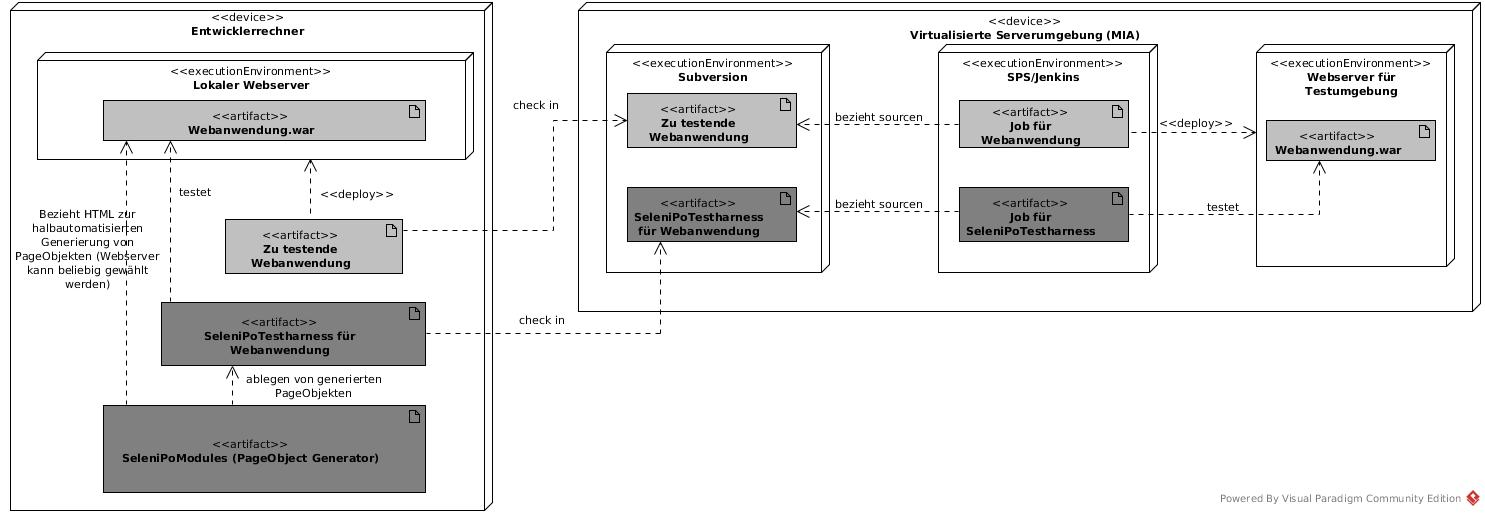
\includegraphics[scale=0.45]{img/Deployment.jpg}\\
  \caption{Einordnung des Page Object Generator in die Deploymentsicht}
  \label{fig:deployment}
\end{figure}

Abbildung \ref{fig:deployment} zeigt die Einordnung des Page Object Generator in die Infrastruktur von it@M. Anhand dieser Abbildung soll gezeigt werden in welchem Bezug sich der Generator zu einer zu testenden Webanwendung und dem späteren Testprojekt befindet.
Zwei übergeordnete Teilbereiche werden unterschieden. Die virtualisierte Serverumgebung (MIA) und der lokale Rechner eines Entwicklers. Auf der virtualisierten Serververumgebung werden die entwicklerübergreifenden Infrastrukturkomponenten wie beispielsweise eine Versionsverwaltung bereitgestellt. Unter dem Entwicklungsrechner ist der Arbeitsplatz eines einzelnen Projektteilnehmers zu verstehen.\\
Auf dem Entwicklungsrechner wird die zu testende Webanwendung entwickelt. Zu Testzwecken kann diese Anwendung in ihrem aktuellen Entwicklungsstand auf einem lokalen Webserver deployt werden.
Der lokale Rechner des Entwicklers ist auch der Ort an dem der Page Object Generator eingesetzt wird. Die lokal deployte Webanwendung kann verwendet werden um für die verschiedenen Seiten der zu testenden Anwendung Page Objects mit Hilfe des Generators zu erzeugen. Diese Page Objects werden in ein zweites Projekt abgelegt, in welchem die Seleniumtestfälle entwickelt werden. Dieses Projekt wird in Abbildung \ref{fig:deployment} als SeleniPoTestharness bezeichnet und kann vom Entwicklerteam entweder selbst erstellt oder als leeres Quickstart-Projekt vorgefertigt bezogen werden. Mit Hilfe der Page Objects im Testharness können Testfälle entwickelt werden die während der Erstellung auf dem lokalen Entwicklungsrechner gegen die lokal deployte Webanwendung ausgeführt werden.
Über die virtualisierte Serverumgebung können die lokal auf den Entwicklungsrechnern der Projektteilnehmer erstellten Ergebnisse zusammengeführt werden. 
Der Sourcecode der zu testende Webanwendung so wie des SeleniPoTestharness wir in einer Versionsverwaltung in der MIA abgelegt. Bei it@M wird zu diesem Zweck Subversion eingesetzt. Über die Versionsverwaltung kann eine Softwareproduktionsstraße bedient werden die das bauen, deployen und testen der der Webanwendung das bisher manuell auf den Entwicklungsrechnern durchgeführt wurde automatisiert. Bei it@M kommt hierfür der Continuous Integration Server Jenkins zum Einsatz. Jenkins bezieht die jeweils aktuellen Sourcen für das Testprojekt und die Webanwendung aus dem Subversion und kann so regelmäßig eine aktuelle Version der Webanwendung bauen und auf ein Testsystem in der virtuellen Serverumgebung deployen. Jenkins kann daraufhin die im Testharness aktuell entwickelten Selenium Testfälle gegen diesen Webserver zur Ausführung bringen.



\subsection{Möglicher Ablauf eines Standartanwendungsfall}
\label{sec:moeglicher_ablauf_eines_standartanwendungsfall}

Abbildung \ref{fig:sequenz} zeigt auf hoher Abstraktionsebene einen Standartablauf bei der Benutzung des Page Object Generators.



\begin{figure}[htb]
  \centering  
  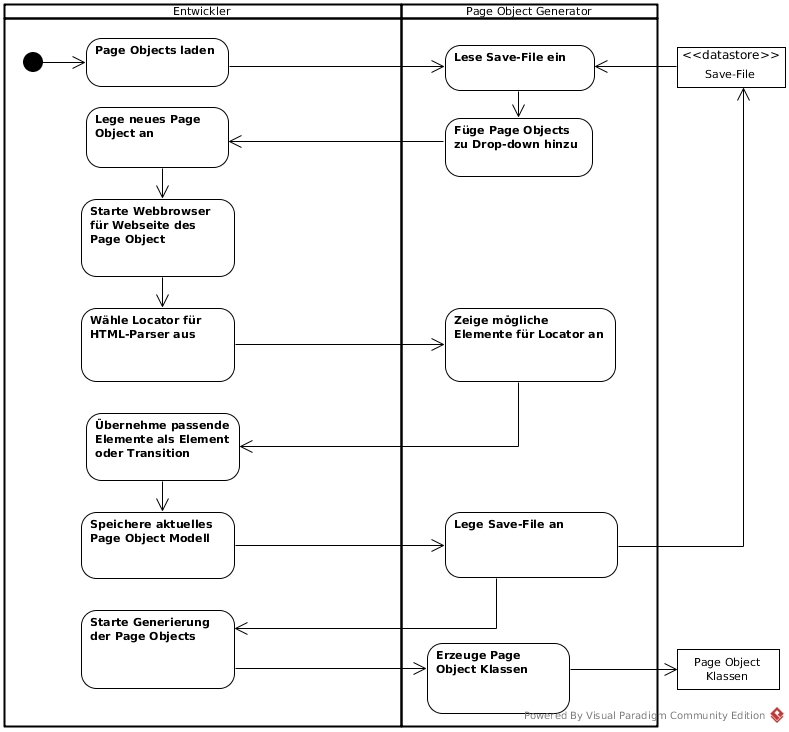
\includegraphics[scale=0.45]{img/Activitydiagram.jpg}\\
  \caption{Möglicher Ablauf eines Standartanwendungsfall}
  \label{fig:sequenz}
\end{figure}

Über das Menü (siehe Abbildung \ref{fig:poGeneratorMenu}) hat der Benutzer des Page Object Generator die Möglichkeit einen bereits zuvor angelegten Zwischenstand des Page Object Modells aus einer XML-Datei zu laden. Die Bereits angelegten Page Objects werden nach dem Laden im Dropdown im bereich des Page Object Modells (siehe Abbildung \ref{fig:poGeneratorPo}) angezeigt. Der Benutzer hat nun die Möglichkeit mit den bereit vorhandenen Page Objects weiterzuarbeiten oder ein neues Page Object anzulegen. Entscheidet er sich dazu, ein neues Page Object anzulegen, wird dieses vorausgewählt im Modell angezeigt. Das Page Object kann nun manuell mit Elemente bzw. Transitionen befüllt werden. Um das Page Object teilautomatisiert zu befüllen kann über den Start-Button ein Webbrowser gestartet werden. Im Browser muss die Seite der Webanwendung geladen werden die dem aktuell ausgewählten Page Object entspricht. Mit dem Dropdown des HTML-Parser (siehe Abbildung \ref{fig:poGeneratorHtml}) kann nun die ausgewählte Webseite nach passenden Elementen bzw. Transitionen durchsucht werden.
Passende Ergebnisse können in das ausgewählte Page Object übernommen und dort bei Bedarf noch einmal überarbeitet werden.
Der neu erreichte Zwischenstand kann wiederum über das Menü gespeichert werden.
Um die Page Objects als Code aus dem Modell zu erzeugen kann über das Menü die Generierung gestartet werden. Bei richtiger Konfiguration des Page Object Generators muss dazu lediglich das Rootverzeichnis des entsprechenden Testprojektes als Zielort der Generierung ausgewählt werden.


\subsection{Anwendungsfälle des Page Object Generator}
\label{sec:page_object_generator_usecases}

Die Anwendungsfälle des Page Object Generators sind in Abbildung \ref{fig:use_case} dargestellt.

\begin{figure}[htb]
  \centering  
  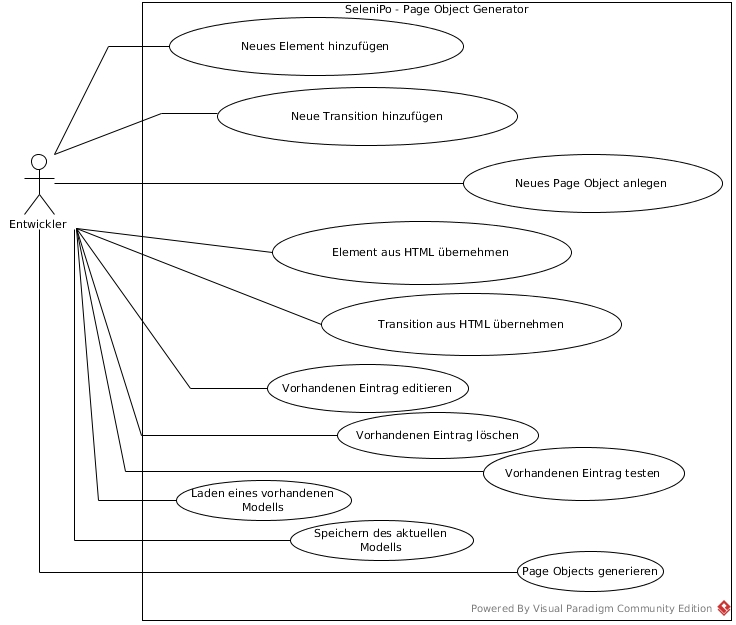
\includegraphics[scale=0.45]{img/Use-Cases.jpg}\\
  \caption{Anwendungsfälle des Page Object Generator}
  \label{fig:use_case}
\end{figure}

Eine detailierte Ausformulierung der Anwendungsfälle befindet sich im Anhang \ref{anhang:anwendungsfallbeschreibung}

\newpage

\subsection{Aufbau des Systems}
\label{sec:aufbau_des_systems}
In seiner internen Struktur ist des Page Object Generator in vier Module aufgeteilt die unterschiedliche aufgaben übernehmen. Auf Projektebene sind diese Module in einem übergeordneten Modul mit dem Namen SeleniPoModules zusammengefasst. Abbildung \ref{fig:component_diagramm} zeigt die verschiedenen Module des Page Object Genrators und deren Abhängigkeiten zueinander.
Neben den Modulen des Page object Generators zeigt Abbildung \ref{fig:component_diagramm} zusätzlich den SeleniPoTestharness der später dazu verwendet werden kann die vom Page Object Generator erzeugten Klassen in einen ausführbaren Kontext zu stellen.

\begin{figure}[htb]
  \centering  
  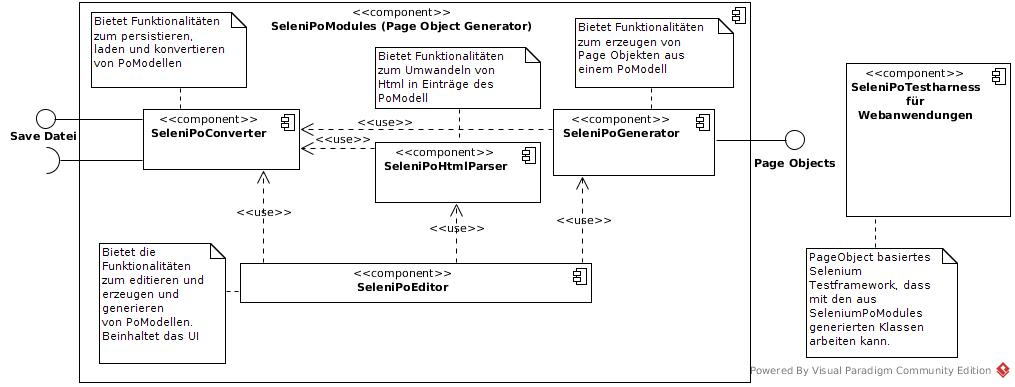
\includegraphics[scale=0.46]{img/ComponentDiagram.jpg}\\
  \caption{Module des Page Object Generators}
  \label{fig:component_diagramm}
\end{figure}

\subsubsection{SeleniPoEditor}
\label{sec:selenipoeditor}

Das zentrale Modul des Page Object Generator ist der SeleniPoEditor.
Ausgehend von diesem Modul werden die übrigen Module verwendet um die in Kapitel \ref{sec:page_object_generator_usecases} vorgestellten Anwendungsfälle zu verwirklichen.
Das Modul SeleniPoEditor stellt dazu das GUI der Anwendung bereit.
Als Technologie wird JavaFX \cite{oracle_client_2015} verwendet das mit der Java Version 1.8 Einzug in den Java Standard gefunden hat. \\
Um eine hohe Wartbarkeit dieser Komponente zu gewährleisten wurde das GUI nach dem Model-View-Controller Prinzip verwirklicht.
Das Model besteht aus einem Anwendungsspezifischem Java Objekt welches eine Liste von Page Objekten mit deren zugehörigen Attributen darstellt.
Für die View wird die XML-basierte Sprache FXML verwendet um losgelöst von der Applikationslogik die Struktur der Benutzeroberfläche zu beschreiben.
Der Controller besteht aus Java Klassen mit deren Hilfe das Verhalten des GUI bei Benutzerinteraktion beschrieben wird.
Komplexere Logik wie beispielsweise das Generieren der fertigen Page Object Klassen wird mittels Services von den übrigen Modulen bereitgestellt.\\
Das Verhalten des GUI wird über einen Zustandsautomaten gesteuert.
Interaktionen mit der Oberfläche beeinflussen den Zustand in dem sich die Anwendung befindet. Je nach Zustand variieren die Aktionen die von den verschiedenen Buttons der Anwendung ausgelöst werden.
Mit Hilfe dieses Prinzieps kann beispielsweise beim auslösen der Editier-Funktion, nach der Auswahl eines Elements, ein anderer Dialog angezeigt werden, als nach der Auswahl einer Transition.
Die verschiedenen Zustände des GUI so wie die Events die in diesen Zuständen verarbeitet werden sind im Anhang \ref{sec:zustände_des_page_object_generator} über einen erweiterten endlichen Automaten dargestellt.

\subsubsection{SeleniPoConverter}
\label{sec:selenipoconverter}
Das Modul SeleniPoConverter dient der Verwaltung des internen Modells des Page Object Generators. In dieser Komponente wird einerseits das Modell der Anwendung definiert andererseits werden Services für andere Module bereit gestellt um mit diesem Modell zu arbeiten.
Abbildung \ref{fig:simple_model} zeigt die Interface-Stuktur welche das Modell abbildet.

\begin{figure}[htb]
  \centering  
  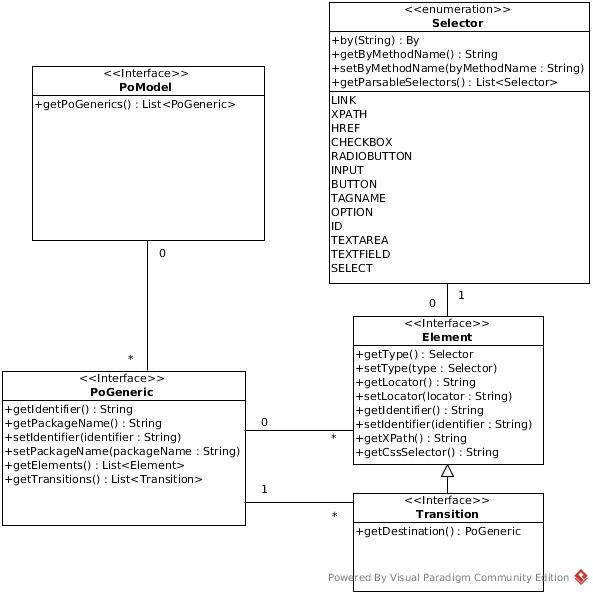
\includegraphics[scale=0.46]{img/SimpleModel.jpg}\\
  \caption{Vereinfachte Struktur des internen Modells des Page Object Generators}
  \label{fig:simple_model}
\end{figure}

Kern des Modells ist das Interface PoModel welches eine Vielzahl von PoGenerics beinhalten kann. Ein PoGeneric repräsentiert die Informationen die benötigt werden um später ein Page Object zu erzeugen. Dementsprechend vereint dieses Interfache eine Menge an Elementen und Transitionen.
Ein Element steht dabei für eine beliebige Komponente einer Webseite wie beispielsweise ein Eingabefeld.
Transitions sind von Elementen abgeleitet. Es handelt sich also um eine speziellere Form von Elementen. Als Transitions werden all die Komponenten einer Webseite bezeichnet die einen Übergang auf ein neues Page Object auslösen. Transitions sind dem zufolge verglichen mit Elementen um ein Ziel Page Object erweitert.
Mit Hilfe von Transitionen ist es Möglich auch die Dynamische Komponente ein Webseite in Form von Seitenübergängen abzubilden.
Sowohl Elemente als auch Transitions werden über einen Selector genauer definiert.
Der Selector gibt für ein Element im Modell an, welche Suchstrategie beim auflösen des Locators gegen die eigentliche Webseite verwendet werden soll.
Die verfügbaren Strategien werden durch die verschiedenen Aufzählungstypen der Enumeration festgelegt.\\
Abbildung \ref{fig:simple_model} zeigt nur die Grundstruktur des zugrunde liegenden Modells. Der Page Object Generator kennt zwei konkrete Implementierungen dieses Modells. Das vollständige Modell ist in Anhang \ref{anhang:vollständiges_technisches_modell} abgebildet.
Zwei verschiedene Implementierungen sind notwendig da JavaFX und XStream \cite{joe_walnes_xstream_2015}, welches für die Persistierung in XML verwendet wird, unterschiedliche Anforderungen an das Modell stellen. JavaFx benötigt spezielle Datentypen wie beispielsweise ObservableList anstelle einer gewöhnlichen List um die View des GUI automatisch mit dem Modell synchron zu halten. Diese Datentypen können von von XStream auf Grund eines fehlenden argumentlosen Konstruktors jedoch nicht mehr deserialisiert werden.
Dementsprechend werden vom Converter eine Reihe von Services bereitgestellt die das Wandeln des Modells in die zwei Implementierungen ermöglicht. Eine Implementierung kann verwendet werden um das Medell zu Persistieren und wieder zu deserialisiert, das andere um im Umfeld von JavaFX zu arbeiten.\\
Abbildung \ref{fig:converter_service} zeigt alle vom Converter bereitgestellten Services. 

\begin{figure}[htb]
  \centering  
  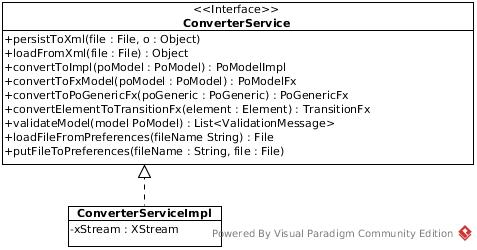
\includegraphics[scale=0.5]{img/ConverterService.jpg}\\
  \caption{Services die von SeleniPoConverter bereitgestellt werden}
  \label{fig:converter_service}
\end{figure}

Neben den Services zum Wandeln des Modells wird in diesem Modul auch die Funktionalität zum speichern und laden so wie zu fachlichen Validierung des Modells bereitgestellt.
Zusätzlich wird die Möglichkeit geboten user-spezifische Informationen wie beispielsweise der Pfad zur zuletzten verwendeten Save-Datei in den Benutzer-Properties abzulegen.


\subsubsection{SeleniPoHtmlParser}
\label{sec:selenipohtmlparser}

Das SeleniPoHtmlParser Modul beinhaltet die Funktionalität zu Teilautomatisierten befüllen von Page Objects mit Elementen bzw. Transitionen.
Das Modul stellt dazu eine Metode bereit die es ermöglicht HTML-Quelltext anhand von einem übergebenen Selector auszuwerten.
Abbildung \ref{fig:html_service} zeigt das Klassendiagramm für diesen Service.

\begin{figure}[htb]
  \centering  
  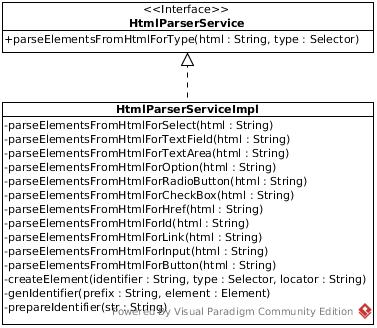
\includegraphics[scale=0.5]{img/HtmlParserService.jpg}\\
  \caption{Services die von SeleniPoHtmlParser bereitgestellt werden}
  \label{fig:html_service}
\end{figure}

Der zu übergebende HTML-Quelltext wird von einen Webbrowser bezogen der über das Modul SeleniPoEditor gestartet werden kann. Zum starten und verwalten dieses Browsers wird wie in den späteren Testfällen Selenium verwendet.
Das Parsing des Quelltext übernimmt die freie Bibliothek jsoup.
Für jeden im Selector definierten Aufzählungstypen wurde dazu eine eigene Strategie implementiert.
Listing \ref{lst:parserLINK} zeigt beispielhaft die Implementierung für den Aufzählungstypen LINK die nur Links auswählt die eines der HTML-Attribute id, text oder title besitzen:
\begin{lstlisting}[caption={Parser für den Aufzählungstypen LINK},label={lst:parserLINK}]
 	/**
	 * Sucht nach Links fuer die vorhanden ist: id or text or title
	 *
	 * @param html Quelltext der zu untersuchenden Seite
	 * @return PoGeneric - neues Page Object mit den gefundenen Elementen
	 */
	private PoGeneric parseElementsFromHtmlForLink(String html) {
		final String PREFIX = "a";
		PoGeneric poGeneric = new PoGenericImpl();
		Document doc = Jsoup.parse(html);
		Elements elements = doc.select("a");
		for (Element element : elements) {
			if (element.hasAttr("id")) {
				de.muenchen.selenipo.Element createdElement = createElement(
						genIdentefier(PREFIX, element), Selector.LINK,
						element.attr("id"));
				poGeneric.getElements().add(createdElement);
			}
			else if (element.hasText()) {
				de.muenchen.selenipo.Element createdElement = createElement(
						genIdentefier(PREFIX, element), Selector.LINK,
						element.text());
				poGeneric.getElements().add(createdElement);
			}
			else if (element.hasAttr("title")) {
				de.muenchen.selenipo.Element createdElement = createElement(
						genIdentefier(PREFIX, element), Selector.LINK,
						element.attr("title"));
				poGeneric.getElements().add(createdElement);
			}
		}
		return poGeneric;
	}
  }
  
\end{lstlisting} 

Die für die jeweiligen Selectoren implementiert Filterstrategie orientiert sich an der Strategie die später in den Testfällen verwendet wird um die Elemente auf der Webseite zu adressieren. Die Testfälle verwenden zum Adressieren der Elemente eine Klasse ByFactory auf die im Abschnitt \ref{sec:selenipotestharness} eingegangen wird.
Dieses vorgehen hat den Nachteil, dass die Möglichkeit besteht, Elemente zu verwerfen die vom Benutzer für den ausgewählten Filter zwar erwartet werden, den implementierten Filterkriterien jedoch nicht entsprechen.
Im Beispiel aus Listing \ref{lst:parserLINK} wären das alle Links für die weder das Attribut id, text oder title gesetzt sind.
Über dieses vorgehen iskt allerdings sichergestellt, dass für einen untersuchten Selector nur Elemente zur Auswahl gestellt werden, die in den späteren Testfällen über die Klasse ByFactory auch aufgelöst werden können.\\
Die Palette der vorgefertigten Filter deckt den größten Teil der im HTML vorhandenen Elemente bereits ab. Sollte es dennoch zu dem Fall kommen, dass Elemente über die existierenden Selectoren nicht erreicht werden können, besteht immer die Möglichkeit mit Hilfe des Selectors XPATH Elemente über einen eigenen XPath-Ausdruck anzusprechen.


\subsubsection{SeleniPoGenerator}
\label{sec:selenipogenerator}
Das Modul SeleniPoGenerator ermöglicht es aus einem Modell des SeleniPoConverters Fertige Page Object Kalssen zu generieren.
Abbildung \ref{fig:generator_service} zeigt das Klassendiagramm des Moduls.

\begin{figure}[htb]
  \centering  
  \includegraphics[scale=0.5]{img/SelenipoGenerator.jpg}\\
  \caption{Services die von SeleniPoHtmlParser bereitgestellt werden}
  \label{fig:generator_service}
\end{figure}
Für die Generierung des Codes aus dem Modell der Anwendung wird die Template-Engine Velocity \cite{apache_software_foundation_apache_2015} verwendet.
Mit Hilfe von Velocity kann ein beliebiges Modell der Anwendung über vordefinierte Templates in die gewünschten Struktur gewandelt werden.
Die Tamplates können vom Benutzer des des Page Object Generators beliebig editiert werden. Auf diese weise können die im Modell der Anwendung hinterlegten Informationen in jede vom Anwender gewünschte Form aufbereitet werden. Anhang \ref{anhang:beispiel_velocity_template} zeigt als Beispiel den Templatevorschlag der im Rahmen dieser Arbeit im Page Object Generator verwendet wird.
Pro Page Object werden jeweils zwei Klassen erzeugt. Listing \ref{lst:template_poeditable}

zwei Teile


\subsubsection{SeleniPoTestharness}
\label{sec:selenipotestharness}

Die Klasse .. wird verwendet um die Möglichkeit zu bieten auch komplexere ausdrücke sinnvoll zu verwalten. Viele tools reduzeiren sich auf einfache ausdrücke die allerdings nicht allzu stabiel sind siehe Kapitel...
Komplexe Ausdrücke über teilweise mehrere zeilen würden die lesbarkeit der Page Objects negativ beeinträchtigen. Über die Klasse ... wurde somit eine möglichkeit geschaffen Komplexere abfragen sinnvoll zu verwalten.


\section{Ausblick}

TODO: 

Technische Sicht. 
Komponentendiagramm Allgemein erklären.

Jede Komponente abarbeiten in sinnvoller tiefe (z.B. Klassendiagram / Zustandsautomat ect.)













